\chapter{Modello di Classificazione}

Per la classificazione dei caratteri estratti dalla fase 1 è stato sviluppato un modello di deep learning. La rete è una Convolutional Neural Network, simile all'architettura LeNet-5: è composta da 2 layer convoluzionali, ognuno dei quali è seguito da un layer di pooling e da una funzione di attivazione ReLU. Dopo i layer convoluzionali, la rete è composta da tre layer fully connected, che producono l'output finale. Per evitare l'overfitting riscontrato sperimentalmente durante l'addestramento, viene utilizzato il dropout tra i layer fully connected.

\begin{figure}[H]
	\centering
	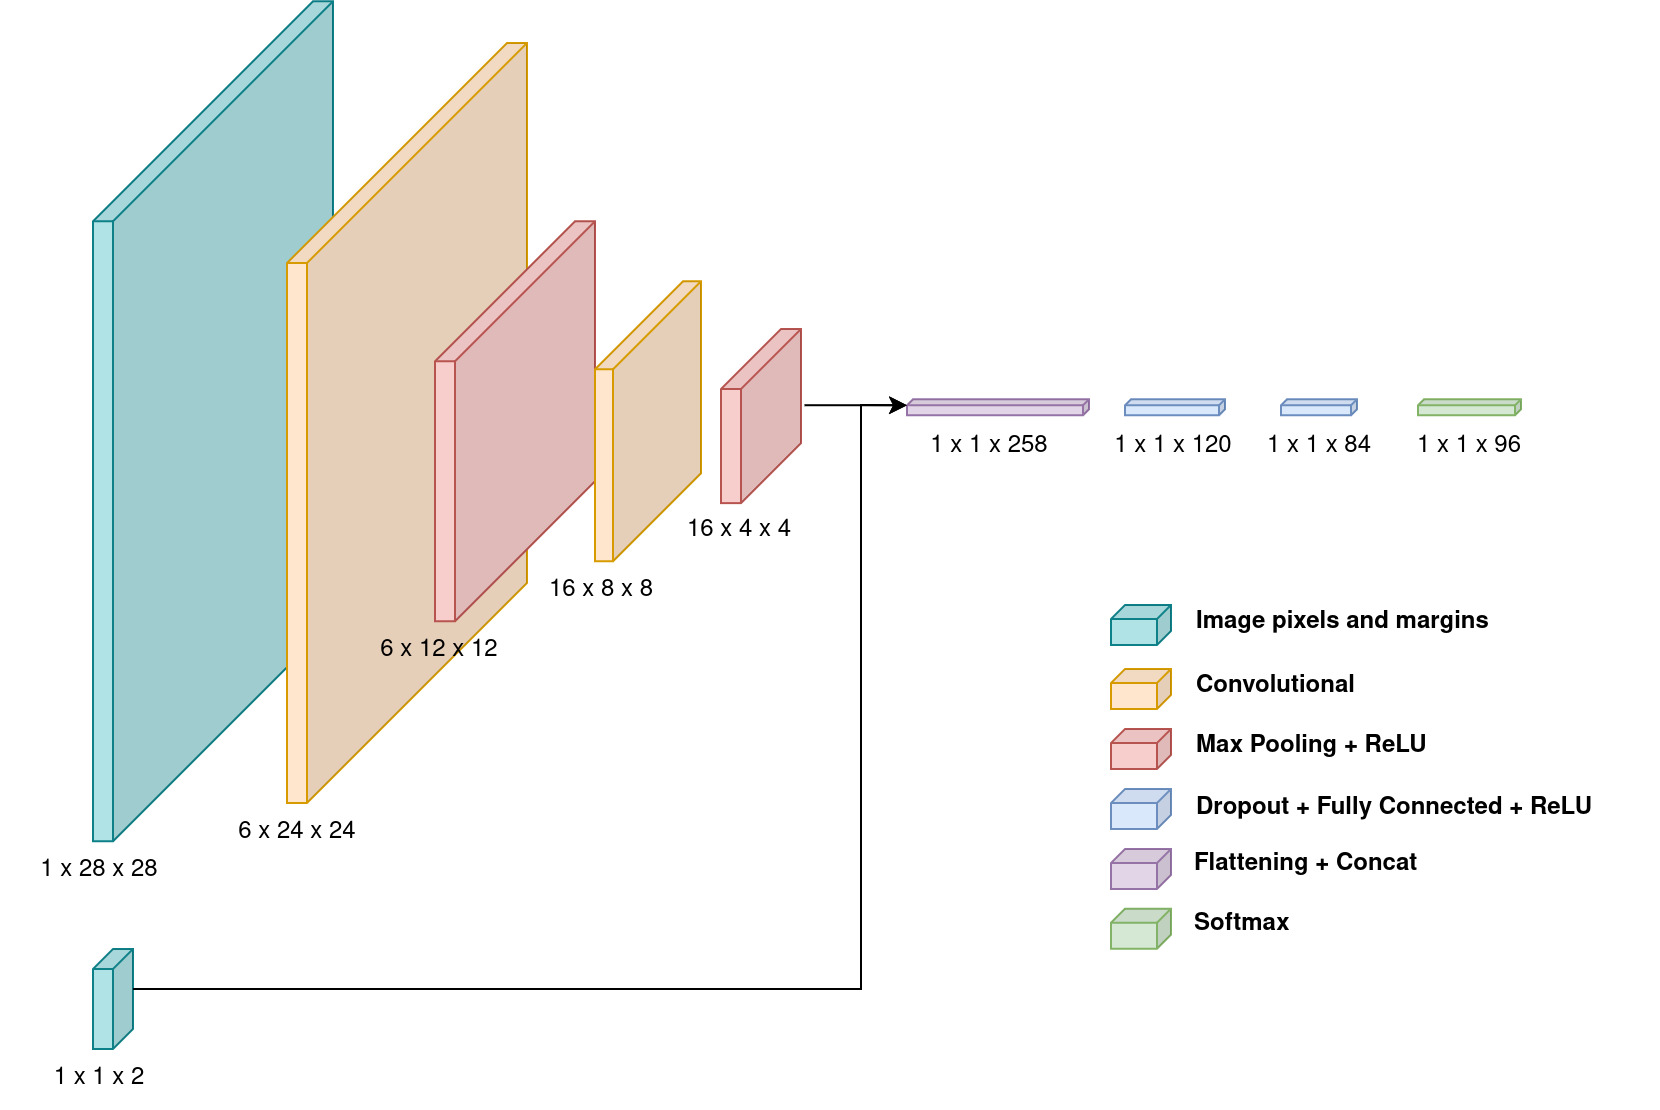
\includegraphics[width=0.8\textwidth]{assets/network.jpg}
	\caption{Schema dell'architettura della rete neurale utilizzata.}
	\label{fig:modello-schema}
\end{figure}
